\documentclass[mathserif]{beamer}
\usepackage[utf8]{inputenc}
\usepackage{tikz}
\usetheme{Szeged}
\usecolortheme{spruce}

\title{Calendar Problem 28}
\subtitle{A line tangent to a circle on the coordinate plane}
\author{Michael Peng}
\date{The Calendar Month, 2018}

\begin{document}
	
	\frame{\titlepage}
	\begin{frame}
		\frametitle{The Problem}
		What is an equation of the line (in y-intercept form) tangent to the graph of $x^2+y^2=25$ at the point $(3,4)$?
		
		\begin{center}
		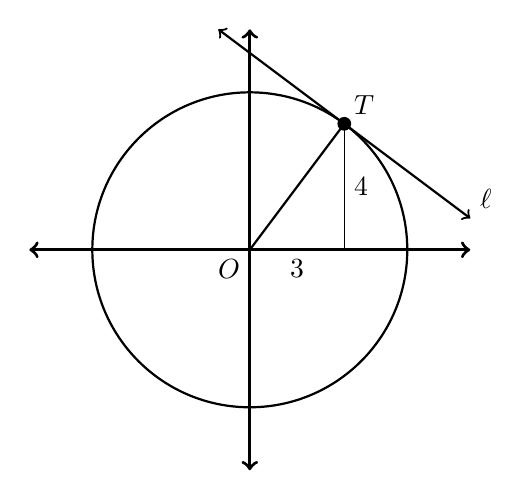
\begin{tikzpicture}[scale=0.4]
		\draw[<->,very thick] (0,7) -- (0,-7);
		\draw[<->, very thick] (-7,0) -- (7,0);
		\draw[thick] (0,0) circle [radius=5];
		\node[below left] at (0,0) {$O$};
		
		\draw[fill] (3,4) circle [radius=0.2];
		\draw (3,4) -- (3,0);
		\node[right] at (3,2) {4};
		\node[below] at (1.5,0) {3};
		\draw[thick] (0,0) -- (3,4);
		
		\draw[<->,thick] (-1,7) -- (7,1);
		\node[above right] at (7,1) {$\ell$};
		\node[above right] at (3,4) {$T$};
		\end{tikzpicture}
		\end{center}
	\end{frame}
\begin{frame}
\frametitle{Prerequisites}
\framesubtitle{11-7}
	\textbf{Given:}  $x^2+y^2=25$\\
	\textbf{Equation for circle:} With center $(h,k)$ and radius $r$, $(x-h)^2+(y-k)^2=r^2$
	
	\bigskip
	
	\begin{tabular}{l | l}
		
		$(x-0)^2+(y-0)^2=25$ & Subtraction Prop. of 0 \\
		$h=0,k=0,r^2=25$ & Matching \\
		$r=\sqrt{25}=5$ & Simplification \\
		The circle is centered at $(0,0)$ & Substitution
		
		\end{tabular}
	
	\bigskip
	
	Name this circle $O$, with center $(0,0)$ and radius $5$.
	\end{frame}
\begin{frame}
\frametitle{Finding Its Slope}
	\begin{columns}[c]
		\begin{column}{.3\textwidth}
			
			\begin{center}
	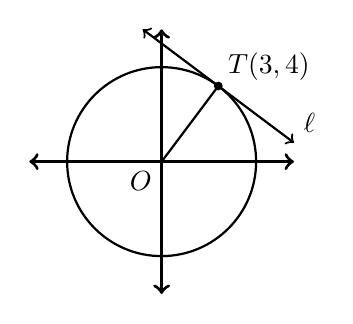
\begin{tikzpicture}[scale=0.24]
	\draw[<->,very thick] (0,7) -- (0,-7);
	\draw[<->, very thick] (-7,0) -- (7,0);
	\draw[thick] (0,0) circle [radius=5];
	\node[below left] at (0,0) {$O$};
	
	\draw[fill] (3,4) circle [radius=0.2];
	\draw[thick] (0,0) -- (3,4);
	
	\draw[<->,thick] (-1,7) -- (7,1);
	\node[above right] at (7,1) {$\ell$};
	\node[above right] at (3,3.8) {$T(3,4)$};
	\end{tikzpicture}
\end{center}
\end{column}
\begin{column}{.7\textwidth}

\renewcommand{\arraystretch}{1.2}
\begin{tabular}{p{4cm} | p{3cm}}
	$\overline{OT}\bot \ell$ & Line tangent to circle $\rightarrow$ line $\bot$ to radius drawn to point of tangency \\
	Slope of $\overleftrightarrow{OT}$ is $\frac{y_2-y_1}{x_2-x_1}$ & Slope Formula \\
	Slope of $\overleftrightarrow{OT}$ is $\frac{4-0}{3-0}=\frac{4}{3}$ & Substitution \\
	Slope of $\ell$ is $-\frac{3}{4}$ & $\bot$ slope is the negative reciprocal
\end{tabular}
\end{column}
\end{columns}
\bigskip
\begin{center}
$\therefore$ The slope of $\ell$ is $-\frac{3}{4}$
\end{center}
\end{frame}
\begin{frame}
\frametitle{Linear Equations}

\textbf{Deduced:}  Slope of $\ell$ is $-\frac{3}{4}$ \\
\textbf{Given:} $\ell$ passes through $T(3,4)$

\bigskip

\textbf{Equation for $\ell$}:
\renewcommand{\arraystretch}{1.2}
\begin{tabular}{l | l}
	$y-4=-\frac{3}{4}(x-3)$ & Point-slope Formula \\
	$y-4=-\frac{3}{4}x-(-\frac{3}{4}\cdot 3)$ & Distributive Property \\
	$y-4=-\frac{3}{4}x+\frac{9}{4}$ & Simplification \\
	$y=-\frac{3}{4}x+\frac{9}{4}+\frac{16}{4}=-\frac{3}{4}x+\frac{25}{4}$ & Addition Prop. of = \\
\end{tabular}
\bigskip
\begin{center}
	 \huge $\boxed{y=-\frac{3}{4}x+\frac{25}{4}}$
\end{center}
\end{frame}
\end{document}